\setauthor{Moritz Eder}
\begin{spacing}{1}
    \chapter*{Abstract}
\end{spacing}
\begin{wrapfigure}{r}{0.3\textwidth}
    \begin{center}
      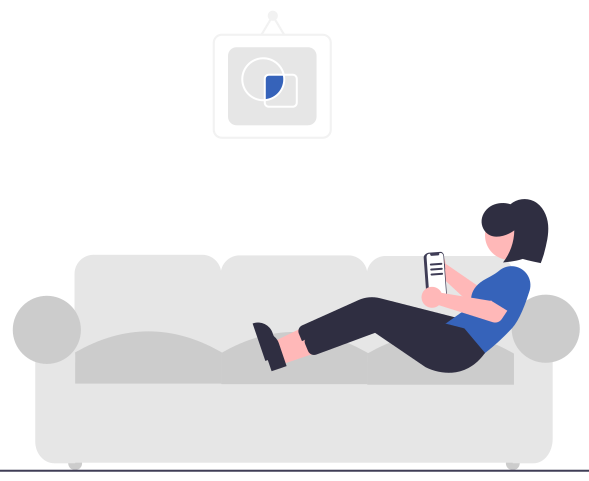
\includegraphics[width=0.3\textwidth]{pics/undraw_Relaxing_at_home_re_mror.png}
    \end{center}
\end{wrapfigure}
In order to give stressed people a simple way to relax, a stress management app has been developed.

Relaxoon is a play on the words 'relax' and 'soon'. Relaxoon offers relaxation exercises in the form of videos, 
texts, articles and more, which are presented in a simple and clear way.

In addition to implementing the front end in React Native and the back end with the content management system
Strapi, the deployment using Kubernetes is described in detail.
\newpage
\begin{spacing}{1}
    \chapter*{Zusammenfassung}
\end{spacing}
\begin{wrapfigure}{r}{0.3\textwidth}
    \begin{center}
      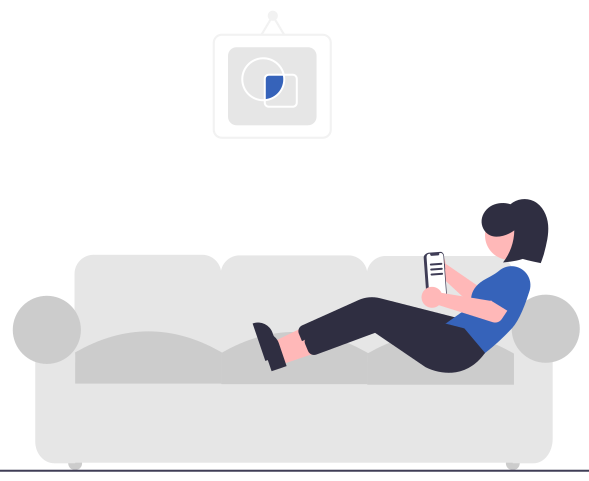
\includegraphics[width=0.3\textwidth]{pics/undraw_Relaxing_at_home_re_mror.png}
    \end{center}
\end{wrapfigure}
Damit gestresste Personen eine simple Möglichkeit haben, sich zu entspannen, wurde eine App zur Stressbewältigung
entwickelt. 

Relaxoon ist ein Wortspiel aus den englischen Wörtern 'relax' und 'soon'. Relaxoon bietet Entspannungsübungen 
in Form von Videos, Texten, Artikeln und mehr, die in einfacher und übersichtlicher Weise dargestellt sind.

Neben der Implementierung des Frontends in React Native und des Backends mit dem Content-Management-System
Strapi wird auf das Deployment mittels Kubernetes im Detail beschreiben.

